\subsection{Строковые абстрактные домены}

Пример простого строкового абстрактного домена реализован в системе \textbf{JSAI}~\cite{guha2012jsai} - платформе статического анализа JavaScript. В ней строки представляются в виде:
\begin{itemize}
    \item любая ($\top$) и неинициализированная ($\bot$) строки
    \item константные строки
    \item категории ``строка-число'', ``спец-символ'' и ``любая строка''
\end{itemize}

\begin{figure}[H]
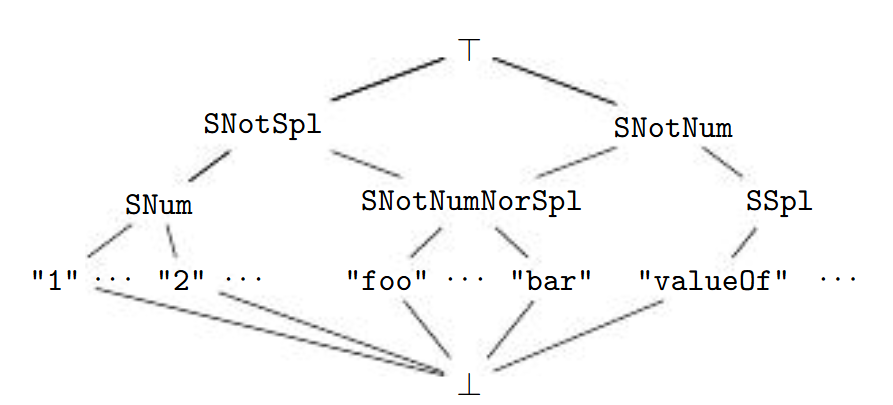
\includegraphics[width=\textwidth]{images/jsai-string-lattice.png}\hfill
\end{figure}


Хотя этот подход обладает высокой производительностью, он страдает от недостатка точности. Например, пусть переменная $s$ может быть равна строке ``foo'' или ``bark''. Тогда значение выражения \texttt{s.length} может быть либо $3$, либо $4$, но абстрактный домен JSAI вернёт «любая длина». Это делает невозможным отбрасывание условий вроде \texttt{if (s.length == 0)} как недостижимых, что ведёт к ложным срабатываниям

\newpage
\begin{lstlisting}[caption={Пример недостаточной точности в строковом домене JSAI}]
let s;
if (input == 0) {
    s = "foo";
} else {
    s = "bark";
}
if (s.length == 0) {
    throw new Error("Divide by zero!");
}
let repeats = 100 / str.length;
\end{lstlisting}

В статьях чаще всего упоминаются ещё 4 строковых решетки

\subsubsection*{The String Set}
Домен множества строк ($SS_k$) сохраняет не более $k$ константных строк. В случае переполнения сбрасывается в $\top$. Этот домен заметно более затратен по времени и памяти. Достаточно просто рассмотреть функцию конкатенации двух абстрактных значений, при которой количество элементов будет произведением. А конкатенация самая часто использующаяся функция на строках, потому от её оптимизации будет многое зависеть

Точность этой решетки очень высокая, так как каждую операцию можно отдельно проделать с каждой строкой в множестве. Но из-за этого и производительность сильно проседает. Плюс теряется вся точность для бесконечного набора возможных строк, который может возникнуть например в цикле при конкатенации

\subsubsection*{The Abstract Length string domain}
Домен длины абстрактной строки ($LS$) запоминает минимальную и максимальную длину строк, которые может принимать абстрактное значение. Например
$$LS("foo"; "bark") = [3, 4] $$
Для примера выше она отлично подойдет, так как запомнит, что минимальная длина 3, а максимальная 4, и даже сможет верно вернуть значение для repeats, то есть интервал [25, 34]. Однако для других операций, таких как substr или charAt, она не годится

\subsubsection*{The Character Inclusion domain}
Домен включения символов ($CI$) отслеживает символы, встречающиеся в строке. Каждая абстрактная строка имеет вид [L, U]. Нижняя граница L содержит символы, которые должны встречаться в конкретной строке (строках), в то время как верхняя граница U представляет символы, которые могут появиться

Этот домен полностью игнорирует структуру конкретных строк, которые аппроксимирует. То есть например 

$$CI("foo") = CI("of") = [\{'f', 'o'\}, \{'f', 'o'\}]$$

Но $CI$, как правило, дешев в вычислительном отношении и иногда предоставляет полезную информацию. Например функция contains, для которой можно вернуть true в случае проверки на включение одной буквы, которая содержится в нижней границе, или же false, если слово содержит букву, которой нет в верхней

\subsubsection*{The Prefix-Suffix domain}
Элементами префикс-суффикс домена ($PS$) являются пары $[p, s]$, содержащие в себе все строки, которые начинаются с p и заканчиваются на s

\[PS("abacab"; "abab") = ["aba"; "ab"]\]

Также как и $CI$, $PS$ не может хранить конкретные строки. Но есть ряд функций, такие как startsWith, endsWith, а иногда и substr, indexOf, для которых будет возвращаться точный ответ в удачных случаях\\

\newpage
\subsection{Конечные автоматы}
Все перечисленные сверху решетки хороши каждая для своего ограниченного набора функций. Но в общем случае будет много неточностей. Поэтому стоит рассмотреть другие подходы, обладающие большей точностью, хоть и более сложные

Для повышения точности анализа был предложен подход, основанный на \textbf{конечных автоматах с переходами по буквам}~\cite{apinis2020symbolic}. В этом подходе множество возможных значений строк моделируется как язык, распознаваемый конечным автоматом. Операции над строками соответствуют операциям над языками: объединение, пересечение, конкатенация и пр.

\subsubsection*{Преимущества}
\begin{itemize}
    \item высокая точность
\end{itemize}

\subsubsection*{Недостатки}
\begin{itemize}
    \item высокая вычислительная сложность
    \item большое потребление памяти
    \item низкая масштабируемость при анализе больших программ
\end{itemize}

\begin{figure}[h]
    \centering
    \begin{tikzpicture}[shorten >=1pt,node distance=1.8cm,on grid,auto]
        \node[state,initial] (q0) {$q_0$};
        \node[state] (q1) [right of=q0] {$q_1$};
        \node[state] (q2) [right of=q1] {$q_2$};
        \node[state,accepting] (q3) [right of=q2] {$q_3$};

        \node[state] (p1) [below of=q1] {$p_1$};
        \node[state] (p2) [right of=p1] {$p_2$};
        \node[state] (p3) [right of=p2] {$p_3$};
        \node[state,accepting] (p4) [right of=p3] {$p_4$};

        \path[->]
          (q0) edge node {f} (q1)
          (q1) edge node {o} (q2)
          (q2) edge node {o} (q3)

          (q0) edge[bend right] node {b} (p1)
          (p1) edge node {a} (p2)
          (p2) edge node {r} (p3)
          (p3) edge node {k} (p4);
    \end{tikzpicture}
    \caption{Конечный автомат, распознающий строки ``foo'' и ``bark''}
\label{fig:automaton}
\end{figure}

Овераппроксимация строк в конечных автоматах повышает точность анализа строк во многих сценариях, но она не подходит для реальных программ, работающих со статически неизвестными входными данными и манипуляциями с длинным текстом




\newpage
\subsection{TARSIS}

TARSIS (Template-based Abstract Representation of Strings with Static analysis) — это современный строковый абстрактный домен, предложенный в работе~\cite{tarsis2021}. Основное новшество Tarsis заключается в том, что он работает с алфавитом строк, а не с отдельными символами. С одной стороны, такой подход требует более сложного и уточненного определения расширяющего оператора и абстрактной семантики строковых операторов. С другой стороны, это позволяет получать более точные результаты

\subsubsection*{Основные функции}
В статье описан алгоритм для аппроксимации с доказательством полноты наиболее часто использующихся функций на строках, а именно length, concat, substr, replace, contains и indexOf

$$\left[ \text{length}(s) \right] = |\sigma|$$
$$\left[ \text{concat}(s, s') \right] = \sigma \cdot \sigma'$$
$$\left[ \text{substr}(s, a, a') \right] = \sigma_i \dots \sigma_j \quad \text{if} \quad i \leq j < |\sigma|$$


\[
\left[ \text{replace}(s, s', s'') \right] = 
\begin{cases}
\sigma \left[ s' / s'' \right] & \text{if } \sigma'  \curvearrowright_s \sigma \\
\sigma & \text{otherwise}
\end{cases}
\]

$$\left[ \text{contains}(s, s') \right] = 
\begin{cases}
\text{true} & \text{if } \exists i, j \in \mathbb{N}. \sigma_i \dots \sigma_j = s' \\
\text{false} & \text{otherwise}
\end{cases}$$

$$\left[ \text{indexOf}(s, s') \right] = 
\begin{cases}
\min \left\{ i \mid \sigma_i \dots \sigma_j = s' \right\} & \text{if } \exists i, j \in \mathbb{N}. \sigma_i \dots \sigma_j = s' \\
-1 & \text{otherwise}
\end{cases}$$

Также важной функцией является widening, при помощи которой удается завершать анализ циклов за конечное время